%!TEX root=paper.tex

\newpage
\section{How Do Students Use the Possibility of Reading Personally Interesting Articles?}
\label{sec:results}

\subsection {Feed Subscriptions}
Figure \ref{fig:registrations} represents an incidence matrix collected at the end of the study interval: the columns represent students, and the rows represent article sources; if a student is registered to a given source, at the intersection of the corresponding row and column we place a $\Diamond$. 

We would expect to see fully continuous horizontal rows of data-points if every user subscribed to the same feed, and fully continuous vertical rows if every user subscribed to all of the feeds available. The fact that these patterns are largely absent in Figure 4 supports our assumption that different individuals prefer to subscribe to different reading sources.

% The figure illustrates that giving the students the freedom to choose the sources they wanted, allowed each one of them to express their interest. 

\begin{figure}[h!]
\centering
  \includegraphics[width=\columnwidth]{figures/users_feeds}
  \caption{Different users subscribe to different sources}~\label{fig:registrations}
\end{figure}

Of course some feeds are more popular than others. Projecting the data- points onto the horizontal axis and sorting the results leaves us with a histogram as can be seen in Figure 5.

\begin{figure}[h!]
\centering
  \includegraphics[width=\columnwidth]{figures/feed_popularity}
  \caption{Some feeds are more popular than others}~\label{fig:registrations}
\end{figure}


{\em 1Jour1Actu} is the most popular article source and Le Figaro - Sant\'e is the least. In order to see whether or not this might be related to how they are presented in the dialog window of our system (see Figure \ref{fig:system_subscriptions}), we can compare the order of popularity with the order in which they are displayed. One can see how the second-to-last presented feed, Le Monde, is the second most popular feed by measure of subscriptions. Conversely, the feed listed above Le Monde is actually the least subscribed-to feed in our listing.


\begin{figure}[h!]
\centering
  \newcommand{\picscale}{0.5}
\newcommand{\yunit}{0.5}
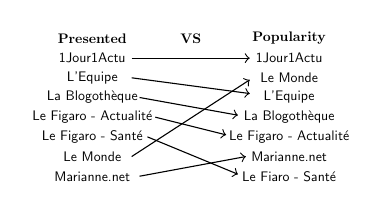
\begin{tikzpicture}[scale=\picscale, every node/.style={scale=\picscale},font=\sffamily]
    % Columns.
    \node at (0  , 0) {\bf Presented};
    \node at (2.5, 0) {\bf VS};
    \node at (5  , 0) {\bf Popularity};
    
    % As presented.
    \node at (0,-1*\yunit) {1Jour1Actu};
    \node at (0,-2*\yunit) {L'Equipe};
    \node at (0,-3*\yunit) {La Blogoth\`{e}que};
    \node at (0,-4*\yunit) {Le Figaro - Actualit\'{e}};
    \node at (0,-5*\yunit) {Le Figaro - Sant\'{e}};
    \node at (0,-6*\yunit) {Le Monde};
    \node at (0,-7*\yunit) {Marianne.net};
    
    % As popular.
    \node at (5,-1*\yunit) {1Jour1Actu};
    \node at (5,-2*\yunit) {Le Monde};
    \node at (5,-3*\yunit) {L'Equipe};
    \node at (5,-4*\yunit) {La Blogoth\`{e}que};
    \node at (5,-5*\yunit) {Le Figaro - Actualit\'{e}};
    \node at (5,-6*\yunit) {Marianne.net};
    \node at (5,-7*\yunit) {Le Fiaro - Sant\'{e}};
    
    % Arrows between presented and popular.
    \draw [->] (1,-1*\yunit)   --   (4,-1*\yunit);
    \draw [->] (1,-2*\yunit)   --   (4,-2.8*\yunit);
    \draw [->] (1.2,-3*\yunit) --   (3.7,-3.9*\yunit);
    \draw [->] (1.6,-4*\yunit) --   (3.4,-4.9*\yunit);
    \draw [->] (1.4,-5*\yunit) --   (3.7,-6.9*\yunit);
    \draw [->] (1,-6*\yunit)   --   (4,-2.1*\yunit);
    \draw [->] (1.2,-7*\yunit) --   (3.9,-6*\yunit);
    
\end{tikzpicture} 
  \caption{The popularity of the feeds vs. their ranking in the UI}~\label{fig:registrations}
\end{figure}




\subsection{Article Interactions}
Figure \ref{fig:articles_read} shows that the articles that the users interact with present a similar pattern: each user explores their own interest, and there is no one article that is interesting for all. The vertical ``line '' in the figure represents an over-active reader.

\begin{figure}[h!]
\centering
  \includegraphics[width=\columnwidth]{figures/users_articles}
  \caption{Every student has their own article reading preferences}~\label{fig:articles_read}
\end{figure}

\subsection{Feature Usage}
\newcommand{\feature}[1]{{\em #1}}
We tracked the usage of the various features in the interactive reader through a telemetry system that records all the interactions with a set of interactive elements of interest. Telemetry is being used increasingly in game design \cite{Gagne11-telemetry} but also in other contexts as a method of user behavior analysis. 

Based on logging every interaction of every user, Figure \ref{fig:feature_usage} shows the six most used features of the system.\footnote{An extended analysis that includes more features is presented elsewhere \cite{Chirtoaca17-apollo}}

  \begin{figure}[h!]
  \centering
    \includegraphics[width=0.9\columnwidth]{figures/reader_feature_usage}
    \caption{Popularity of features by their recorded usage-events}
    \label{fig:feature_usage}
  \end{figure}

With 6.700 occurrences, \feature{requesting a translation for a word} is the most used interactive feature of the system. The second most used feature is \feature{opening the translation alternatives} drop-down list. The six-to-one ration between the two features is an indicator of the limitations of the automatic translation -- it seems that one in six translations are not satisfying to the learners.

The third most used feature is \feature{pronounciation}. On average, there are about 1.66 pronunciations for a given translation, suggesting that users are often asking for a second pronunciation after hearing it the first time. 

% \ml{@dan, do you agree with this conclusion? it's opposite to your thesis, but I think this is the correct interpretation}

% In addition, we looked at the number of times the same word or phrase was pronounced by the same user. This data ranges from one single pronunciation to 14 pronunciations for the same word (phrase). The size of this interval is mostly due to the users' different proficiency in a certain language and the difficulty in pronunciation of the word (phrase) itself. Nevertheless, on average, the number approaches 1.66 pronunciation requests for the same piece of text, suggesting that users are generally sufficiently content with a pronunciation after hearing it the first time.


\feature{Undo}-ing a translation is used when the user wants to remove the last translation that was inserted in the text. For the proposed interaction mechanism this feature seems to be useful. 

A {\em like} button found at the bottom of an article  was clicked by the readers 174 times. Although not used at the moment, this information can be used in the future to improve article recommendations.
 % and maybe to add a social dimension to the system by providing information about how other people react to a given article.

The least used feature presented in the Figure \ref{fig:feature_usage}, {\em translation suggestion}, allows users to contribute their own translations when they are not satisfied with the one automatically provided by the system. 
% \ml{which brings me to: @Dan, what do you mean by alternatives here? :) Is it the number of times somebody selected an alternative, or the number of times they opened the menu. In any case, can we get the other number?}

  \begin{figure}[h!]
  \centering
    \includegraphics[width=0.9\columnwidth]{figures/reader_feature_usage_per_user}
    \caption{The usage of the various reader features by the various users }
    \label{fig:usage_per_user}
  \end{figure}


Figure \ref{fig:usage_per_user} shows the number of distinct users for each category of events. A larger number of distinct users indicates a feature that is more important to the students. We see that: 
\begin{itemize}
  \item not all the users of the system use translations
  \item \feature{translation suggestion} is used by very few users. It still is to be determined whether this is due to readers overwhelmingly being satisfied with the automatic translations and their alternatives, or due to a low involvement. 
\end{itemize}



\newpage
\section{How Do Students Use the Personalized Vocabulary Exercises?}

The system presented four types of vocabulary practice exercises to the students. In total, during the entire duration of the study we observed 18.082 exercises being presented to the students. Figure \ref{fig:ex_interactions} presents the number of exercises which had a ``correct'' outcome (red) vs. exercises which had a ``wrong'' outcome (blue). The figure shows one student who did 3.000 (!) exercises during one month, and about six over-eager students who did more than 700 exercises. 

  \begin{figure}[h!]
  \centering
    \includegraphics[width=\columnwidth]{figures/exercise_interactions_count.png}
    \caption{Correct (red) and wrong (blue) exercise outcomes per student}
    \label{fig:ex_interactions}
  \end{figure}

The figure does not include one other type of outcome, {\em requesting a hint}, which is presented in the table below grouped per exercise type. The corresponding number of hints suggests that the multiple-choice exercises (i.e. Match, Choose) are simpler than free text entry exercises (i.e. Find, Translate).

\begin{tabular}{lrrrr}
  % source id: 
  % choose -- 5
  % find -- 4
  % translate -- 7
  % match -- 6
                      & Choose  & Find & Translate & Match \\ \hline
  Total interactions  & 7180    & 6249 & 2643      & 2010\\
  Hint requests       & 29      & 529  & 847       & 16 \\ \hline
  \label{tab:hints_per_ex_type}
\end{tabular}

Figure \ref{fig:activity_per_day} shows the days when learners practice exercises. It suggests constant activity over the entire period of the study with a more intensive period towards the end.

  \begin{figure}[h!]
  \centering
    \includegraphics[width=0.8\columnwidth]{figures/user_exercise_activity_vs_day.pdf}
    \caption{The students are doing exercises at their own pace throughout the one month interval }
    \label{fig:activity_per_day}
  \end{figure}

\newpage
\section{What is the Perception of the Learners?}

\subsection{In App Feedback Request}
Besides the analysis that we did based on the observed user data, we also asked the students a series of questions by popping up questions while they are using the sytem (by using an online tool called HotJar). Among the questions was whether they preferred the reading platform and why. Some of the qnswers can be seen in the screenshot below. It becomes clear that the students appreciate the possibility of reading what is interesting for them.

    \begin{figure}[h!]
    \centering
      \includegraphics[width=0.9\columnwidth]{figures/opinion_on_reading_platform}
      \caption{The students appreciate the freedom of reading what is interesting to them }
    \end{figure}

\subsection{Post-Usage Survey}

The majority of the students who answered our post-usage survey said that  they prefer our system to a textbook. However, we still think this is not very conclusive since the number of students who answered our survey was quite limited: 12 of the 60 students represent about 20\% of the participants. 


\subsection{Reports to the Teacher}
However, since they might have been more sincere when reporting to their teacher than directly to us, we report here also what they wrote in a separate evaluation of the tools they use in the class, which the teacher runs always at the end of the school year. Several of the answers are: 

\begin{description}
  \item {\em ``It works well but it were better if the translation would have been in Dutch. It is good that you can choose yourself what to read.''}
  \item {\em ``Good for reading skills. It would have been best if it were in Dutch.''}
  \item {\em ``Your vocabulary is really moving forward, but then you have to do it more often than a few times. Overall a nice website, easy and fun subjects''}
\end{description}

There main message in the feedback is that learners appreciate the freedom of chosing materials to read that are personally interesting for them. The second, implied observation is that they appreciate the translations, but they would want to have them in their native language. 

% The way forward is then, by providing better recommendations if possible, and by providing translations in their native languages.

% In the future we plan to investigate whether the system works well enough with Dutch.

\newpage
\section{Limitations of this Study}
\label{sec:limitations}
% We presented a system, and we showed that it has the potential to generate user involvement. However the study we performed is not sufficient to reach a strong conclusion about the impact of the system we present... 

The feedback from the users was positive. However, they might have been influenced by our enthusiastic presentation of the system at the begining of the testing month. 



We showed that the users are using the system extensively. However, this might be because the students had to use the system as part of their assignment in the class. We showed that the majority of the students used the system constantly throughout the one month period. If they only used it for a grade, we would have expected a more focused cramming at the end of the period (which we actually saw with a few of the students, but not with the majority). 

The students we worked with are not necesarily representative for the Dutch highschool student population since they are bilingual. Even in this case, during the fedback multiple of them opined that they would prefer to use the system in their native Dutch as opposed to English.

% We observed that students prefer to interact with different texts...  

The algorithms for scheduling vocabulary exercises are the state of the art in spaced repetition. However, we did not have a control group to see whether this approach works better than others. Moreover, note that other approaches for using spaced repetition already exist; what is unique in our approach is that the students learn based on personalized exercises generated based on the context of their past readings.






